
\documentclass[conference]{IEEEtran}

\usepackage{cite}
\usepackage{amsmath,amssymb,amsfonts}
\usepackage{algorithmic}
\usepackage{graphicx}
\usepackage{textcomp}
\usepackage{bm}
\usepackage{upgreek}

%\usepackage[retainorgcmds]{IEEEtrantools}

\usepackage[nottoc]{tocbibind}


\linespread{1.3}


\title{Predictive Distribution Estimation for Bayesian Machine Learning using a Dirichlet Process Prior}

%\author{Paul Rademacher}
\author{
\IEEEauthorblockN{Paul Rademacher}
\IEEEauthorblockA{U.S. Naval Research Laboratory\\Radar Division\\Washington, DC 20375, USA}
\and
\IEEEauthorblockN{Milo\v{s} Doroslova\v{c}ki}
\IEEEauthorblockA{The George Washington University\\Department of Electrical and Computer Engineering\\Washington, DC 20052, USA}
}


%\graphicspath{ {C:/Users/Paul/Documents/PhD/Dissertation/Documentation/Figures/} }
\graphicspath{ {../Figures/} }


\DeclareMathOperator*{\argmin}{arg\,min}
\DeclareMathOperator*{\argmax}{arg\,max}

\DeclareMathOperator{\xrm}{\mathrm{x}}
\DeclareMathOperator{\Xrm}{\mathrm{X}}
\DeclareMathOperator{\yrm}{\mathrm{y}}
\DeclareMathOperator{\Yrm}{\mathrm{Y}}
\DeclareMathOperator{\Drm}{\mathrm{D}}
\DeclareMathOperator{\nrm}{\mathrm{n}}
\DeclareMathOperator{\nbarrm}{\bar{\mathrm{n}}}
\DeclareMathOperator{\zrm}{\mathrm{z}}

\DeclareMathOperator{\Prm}{\mathrm{P}}
\DeclareMathOperator{\prm}{\mathrm{p}}
\DeclareMathOperator{\Erm}{\mathrm{E}}
\DeclareMathOperator{\Crm}{\mathrm{C}}

\DeclareMathOperator{\Xcal}{\mathcal{X}}
\DeclareMathOperator{\Ycal}{\mathcal{Y}}
\DeclareMathOperator{\Dcal}{\mathcal{D}}
\DeclareMathOperator{\Ncal}{\mathcal{N}}
\DeclareMathOperator{\Zcal}{\mathcal{Z}}
\DeclareMathOperator{\Hcal}{\mathcal{H}}
\DeclareMathOperator{\Fcal}{\mathcal{F}}
\DeclareMathOperator{\Rcal}{\mathcal{R}}
\DeclareMathOperator{\Mcal}{\mathcal{M}}
\DeclareMathOperator{\Scal}{\mathcal{S}}
\DeclareMathOperator{\Pcal}{\mathcal{P}}
\DeclareMathOperator{\Lcal}{\mathcal{L}}

\DeclareMathOperator{\Rbb}{\mathbb{R}}
\DeclareMathOperator{\Nbb}{\mathbb{N}}
\DeclareMathOperator{\Zbb}{\mathbb{Z}}

\DeclareMathOperator{\Dir}{\mathrm{Dir}}
\DeclareMathOperator{\DM}{\mathrm{DM}}
\DeclareMathOperator{\Mult}{\mathrm{Mult}}
\DeclareMathOperator{\DP}{\mathrm{DP}}









\begin{document}

\maketitle

\begin{abstract}
In Bayesian treatments of machine learning, the success or failure of the estimator/classifier hinges on how well the prior distribution selected by the designer matches the actual data-generating model. This paper assumes that the data-generating PMF is a realization of a Dirichlet process and assesses the mismatch between the true predictive distribution and the predictive distribution approximated using the training data. It is shown that highly localized Dirichlet priors can overcome the burden of a limited training set when the prior mean is well matched to the true distribution, but will degrade the approximation if the match is poor. A bias/variance tradeoff will be demonstrated with illustrative examples.
\end{abstract}



\section{Extended Summary}

This article investigates how a Bayesian perspective influences the predictive distributions used to make decisions in machine learning applications. The efficacy of Bayesian learning methods depends on how well the prior knowledge imparted by the designer matches the true data-generating PMF $\uptheta$. The chosen prior distribution $\prm_\uptheta$ over the set of data-generating probability mass functions (PMF) reflects the users confidence that different PMF's $\uptheta$ are responsible for generating the novel pair $(\yrm,\xrm) \in \Ycal \times \Xcal$ and the observed training data $\Drm = (\Yrm,\Xrm) \in \Dcal = \{\Ycal \times \Xcal\}^N$. The elements $(\yrm,\xrm)$ are characterized by $\Prm_{\yrm,\xrm | \uptheta}(y,x | \theta) = \theta(y,x)$ and the training data by
\begin{IEEEeqnarray}{rCl}
\Prm_{\Drm | \uptheta}\big( D | \theta \big) & = & \prod_{n=1}^N \theta \big(Y_n,X_n \big) \\
& = & \prod_{y \in \Ycal} \prod_{x \in \Xcal} \theta(y,x)^{\bar{N}(y,x;D)} \nonumber \;.
\end{IEEEeqnarray}
The dependency on $\Drm$ is expressed though the function
\begin{IEEEeqnarray}{rCl}
\bar{N}(y,x;D) & = & \sum_{n=1}^N \delta \left[ y,Y_n \right] \delta \left[ x,X_n \right] \;,
\end{IEEEeqnarray}
where $\delta[\cdot,\cdot]$ is the Kronecker delta function. The random elements $\xrm$ and $\Drm$ are observable and provide predictive information about the unobserved value of $\yrm$.

If a highly localized prior distribution $\prm_\uptheta$ is chosen that strongly weights the actual data PMF, low risk learning functions are possible even with limited training data $\Drm$; however, if the true PMF's weighting is low, a good solution will never be achieved. Conversely, a high-variance prior PDF leads to decision functions that will always be able to adapt with enough training data; if data is limited, however, the function may not deliver the required performance.

This article assumes that the data-generating PMF is a realization of a Dirichlet process. The Dirichlet distribution for the PMF model $\uptheta \in \Theta$ is \cite{bishop}
\begin{IEEEeqnarray}{rCl}
\prm_\uptheta(\theta) & = & \beta(\alpha)^{-1} \prod_{y \in \Ycal} \prod_{x \in \Xcal} \theta(y,x)^{\alpha(y,x) - 1} \;,
\end{IEEEeqnarray}
where the user-selected PDF parameters $\alpha : \Ycal \times \Xcal \mapsto \Rbb^+$ are introduced and $\beta$ is the generalized beta function.

The class of Dirichlet probability density functions (PDF) have the desirable properties of full support over the set of possible PMF's and a tractable posterior distribution for independently and identically distributed data \cite{ferguson}. 

Additionally, control of the Dirichlet parameters can enable both maximally and minimally localized prior distributions. The parameters $\alpha$ control around which models $\uptheta$ the PDF concentrates and how strongly. For convenience, introduce the concentration parameter $\alpha_0 \equiv \sum_{y \in \Ycal} \sum_{x \in \Xcal} \alpha(y,x)$. 

Of specific interest is how $\prm(\uptheta)$ changes as the concentration parameter approaches its limiting values. For $\alpha_0 \to \infty$, the PDF concentrates at its mean, resulting in
\begin{IEEEeqnarray}{rCl}
\prm_\uptheta(\theta) & = & \delta\left( \theta - \frac{\alpha}{\alpha_0} \right) \;,
\end{IEEEeqnarray}
where $\delta(\cdot)$ is the Dirac delta function over the set $\Theta$. Conversely, for $\alpha_0 \to 0$, the PDF trends toward
\begin{IEEEeqnarray}{rCl}
\prm_\uptheta(\theta) & = & \sum_{y \in \Ycal} \sum_{x \in \Xcal} \frac{\alpha(y,x)}{\alpha_0} \delta\big( \theta - \delta[\cdot,y] \delta[\cdot,x] \big) \;,
\end{IEEEeqnarray}
which distributes its weight among the $|\Ycal| |\Xcal|$ models with an $\ell_0$ norm satisfying $\| \theta \|_0 = 1$. These trends are demonstrated in Figure \ref{fig:P_theta}. 
\begin{figure}
\centering
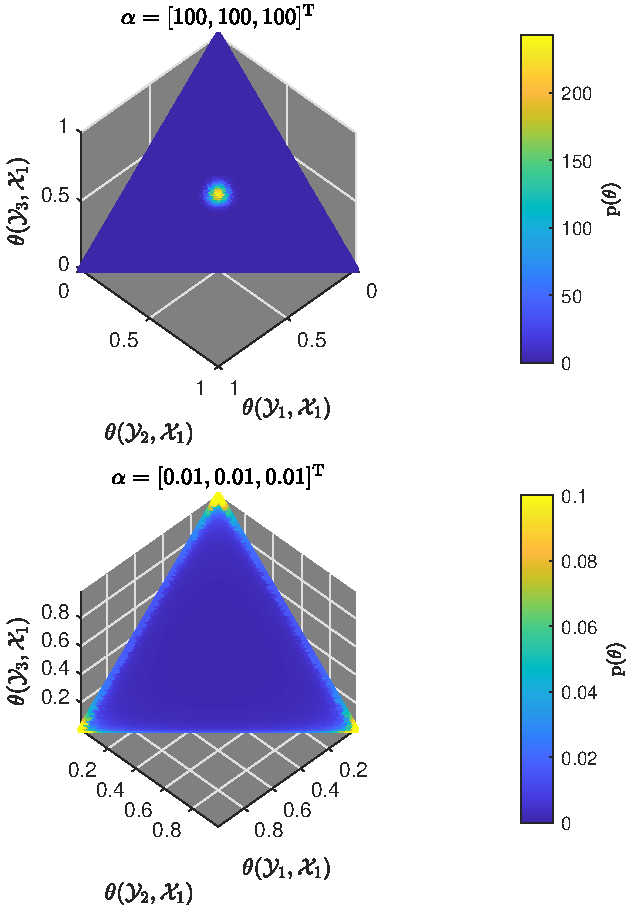
\includegraphics[width=1\linewidth]{P_theta.pdf}
\caption{Model prior PDF $\prm(\uptheta)$ for different concentrations $\alpha_0$}
\label{fig:P_theta}
\end{figure}



Define the decision function $f: \Dcal \mapsto \Hcal^{\Xcal}$, where $\Hcal$ is the decision space. The metric guiding the design is the conditional expected loss, or conditional ``risk'',
\begin{equation} \label{eq:risk_cond}
\Rcal_{\Theta}(f ; \uptheta) = \Erm_{\Drm | \uptheta} \bigg[ \Erm_{\yrm,\xrm | \uptheta} \Big[ \Lcal\big( f(\xrm,\Drm),\yrm \big) \Big] \bigg] \;,
\end{equation}
where $\Lcal: \Hcal \times \Ycal \mapsto \Rbb_{\geq 0}$ is the user-specified loss function. 



If the model $\uptheta$ were observable, a ``clairvoyant'' decision function $f_{\Theta}: \Theta \mapsto \Hcal^{\Xcal}$ could be designed that is dependent only on the true predictive distribution $\Prm_{\yrm | \xrm,\uptheta}$. However, as the model $\uptheta$ is unknown, the prior distribution $\prm_{\uptheta}$ is assumed and the Bayes risk can be formulated as
\begin{IEEEeqnarray}{rCl} \label{eq:risk}
\Rcal(f) & = & \Erm_{\uptheta}\Big[ \Rcal_{\Theta}\big( f(\xrm,\Drm) ; \uptheta \big) \Big] \\
& = & \Erm_{\xrm,\Drm}\bigg[ \Erm_{\yrm | \xrm,\Drm} \Big[ \Lcal\big( f(\xrm,\Drm),\yrm \big) \Big] \bigg] \nonumber \;.
\end{IEEEeqnarray}
Now, the decision function is dependent on the predictive distribution 
\begin{IEEEeqnarray}{rCl}
\Prm_{\yrm | \xrm,\Drm}(y | x,D) & = & \frac{\alpha(y,x) + \bar{N}(y,x;D)}{\alpha'(x) + N'(x;D)} \\
& = & \left(\frac{\alpha'(x)}{\alpha'(x) + N'(x;D)}\right) \frac{\alpha(y,x)}{\alpha'(x)} \nonumber \\
&& \quad + \left(\frac{N'(x;D)}{\alpha'(x) + N'(x;D)}\right) \frac{\bar{N}(y,x;D)}{N'(x;D)} \nonumber \;,
\end{IEEEeqnarray}
where $\alpha'(x) \equiv \sum_{y \in \Ycal} \alpha(y,x)$ and $N'(x;D) = \sum_{n=1}^N \delta \left[ x,X_n \right]$. This PMF can be interpreted as an estimate of the true predictive distribution $\Prm_{\yrm | \xrm,\uptheta}$.

It is informative to compare the Bayesian predictive distribution $\Prm_{\yrm | \xrm,\Drm}$ to the unobserved predictive PMF $\Prm_{\yrm | \xrm,\uptheta}$ and investigate the effects of the Dirichlet prior localization. As $\bar{N}(\Drm)$ is a sufficient statistic for the PMF $\uptheta$, any distributions dependent on $\Drm$ will be replaced by their corresponding distributions of $\nbarrm \equiv \bar{N}(\Drm)$, simplifying the analysis. Note that $\nbarrm | \uptheta \sim \Mult(N,\uptheta)$ \cite{theodoridis-ML}.

For a given observation $\xrm = x$ and corresponding number of training samples $\nrm'(x) \equiv \sum_{y \in \Ycal} \nbarrm(y,x)$, the expected value of the predictive PMF estimate condtioned on the true model $\uptheta$ is
\begin{IEEEeqnarray}{L}
\Erm_{\nbarrm | \nrm',\uptheta}\big[ \Prm_{\yrm | \xrm,\nbarrm}(y | x,\nbarrm) \big] \\ 
\quad = \left(\frac{\alpha'(x)}{\alpha'(x) + \nrm'(x)}\right) \frac{\alpha(y,x)}{\alpha'(x)} + \left(\frac{\nrm'(x)}{\alpha'(x) + \nrm'(x)}\right) \frac{\uptheta(y,x)}{\uptheta'(x)} \nonumber \;.
\end{IEEEeqnarray}
where the aggregation property for multinomial distributions has been used \cite{johnson}. 

To aid further characterization of the Bayesian predictive distribution, define the difference between the estimated and true predictive PMF's as the random process $\Delta(\cdot;x,\nbarrm) \equiv \Prm_{\yrm | \xrm,\nbarrm}(\cdot | x,\nbarrm) - \Prm_{\yrm | \xrm,\uptheta}(\cdot | x,\uptheta)$. Given $\xrm = x$ and a corresponding number of training samples $\nrm'(x)$, the bias of the conditional PMF estimate is
\begin{IEEEeqnarray}{rCl}
\mathrm{Bias}(y;x,\nrm') & = & \Erm_{\nbarrm | \nrm',\uptheta}\big[ \Delta(y;x,\nbarrm) \big] \\
& = & \frac{\alpha'(x)}{\alpha'(x) + \nrm'(x)} \left( \frac{\alpha(y,x)}{\alpha'(x)} - \frac{\uptheta(y,x)}{\uptheta'(x)} \right) \nonumber 
\end{IEEEeqnarray}
and its covariance function is 
\begin{IEEEeqnarray}{L}
\mathrm{Cov}(y,y';x,\nrm') = \Crm_{\nbarrm | \nrm',\uptheta} \big[\Prm_{\yrm | \xrm,\nbarrm}(\cdot | x,\nbarrm) \big](y,y') \\
\quad = \frac{\nrm'(x)}{\big( \alpha'(x) + \nrm'(x) \big)^2} \left( \frac{\uptheta(y,x)}{\uptheta'(x)} \delta[y,y'] - \frac{\uptheta(y,x)}{\uptheta'(x)} \frac{\uptheta(y',x)}{\uptheta'(x)} \right) \nonumber \;,
\end{IEEEeqnarray}
where $C$ is the covariance operator for functions of random elements.

Combining the estimator bias and variance, the conditional second moments of $\Delta(\cdot;x,\nbarrm)$ are
\begin{IEEEeqnarray}{L}
\mathcal{E}(y,y' ; x,\nrm') = \Erm_{\nbarrm | \nrm',\uptheta} \Big[ \Delta(y;x,\nbarrm) \Delta(y';x,\nbarrm) \Big] \\
\qquad = \mathrm{Bias}(y;x,\nrm') \mathrm{Bias}(y';x,\nrm') + \mathrm{Cov}(y,y';x,\nrm') \nonumber \;.
\end{IEEEeqnarray}

To exemplify how the model estimate $\Prm_{\yrm | \xrm,\Drm}$ approximates $\Prm_{\yrm | \xrm,\uptheta}$, consider a scenario with $|\Ycal| = 10$. The data-independent PMF $\alpha / \alpha_0$ and true model $\uptheta$ are shown in Figure \ref{fig:P_yx_error_N_0} - note the significant mismatch. 

Figures \ref{fig:P_yx_error_a0_0_1} and \ref{fig:P_yx_error_a0_10} show how the expected value and variance of the PMF estimate (represented by the blue markers and error bars) change for different values of $\nrm'(x)$ and $\alpha'(x)$. Note that the upper and lower error bars represent the expected squared deviation above and below the conditional mean $\Erm_{\nbarrm | \nrm',\uptheta}\big[ \Prm_{\yrm | \xrm,\nbarrm}(y | x,\nbarrm) \big]$, respectively. Each individual plot heading provides the error $\sqrt{\sum_{y \in \Ycal} \mathcal{E}(y,y ; x,\nrm')}$ to assess the quality of the PMF estimate. 

Observe that for $\nrm'(x) = 1$, the high variance of the $\alpha'(x) = 0.1$ estimate (favoring the empirical PMF) renders it worse than the $\alpha_0 = 10$ estimate; in fact, the variance is so high that the error exceeds that of the data-independent estimate $\alpha(\cdot,x) / \alpha'(x)$ (Figure \ref{fig:P_yx_error_N_0}). Conversely, for $\nrm'(x) = 10$, the confidence of the $\alpha'(x) = 10$ estimate leads to high bias and the $\alpha'(x) = 0.1$ estimate is superior. For $\nrm'(x) = 100$, both the $\alpha'(x) = 0.1$ and $\alpha'(x) = 10$ estimates begin converging to the true predictive distribution - this is guaranteed due to the full support of the Dirichlet prior.


\begin{figure}
\centering
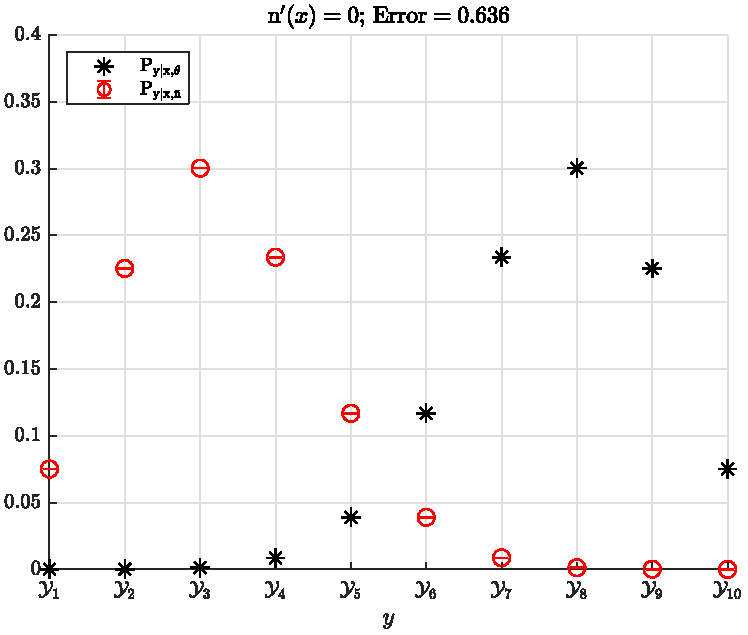
\includegraphics[width=1\linewidth]{P_yx_error_N_0.pdf}
\caption{Model $\uptheta$ estimate, no training data}
\label{fig:P_yx_error_N_0}
\end{figure}

\begin{figure}
\centering
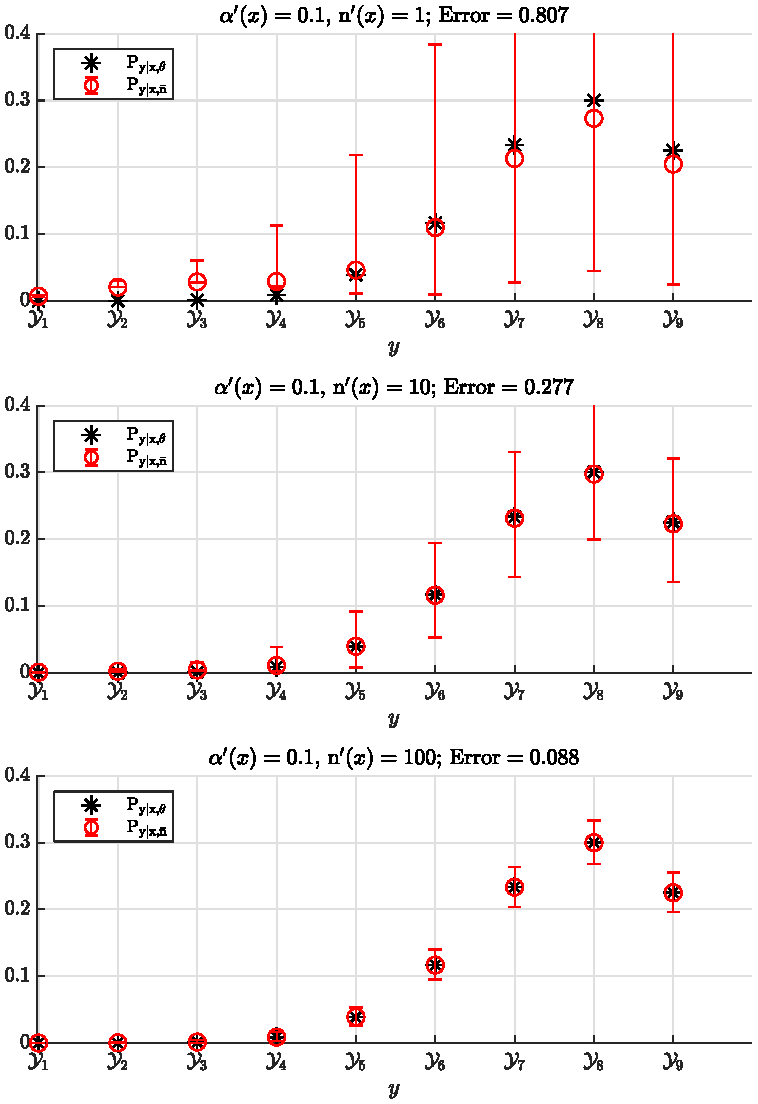
\includegraphics[width=1\linewidth]{P_yx_error_a0_0_1.pdf}
\caption{Model $\uptheta$ estimates, $\alpha_0 = 0.1$}
\label{fig:P_yx_error_a0_0_1}
\end{figure}

\begin{figure}
\centering
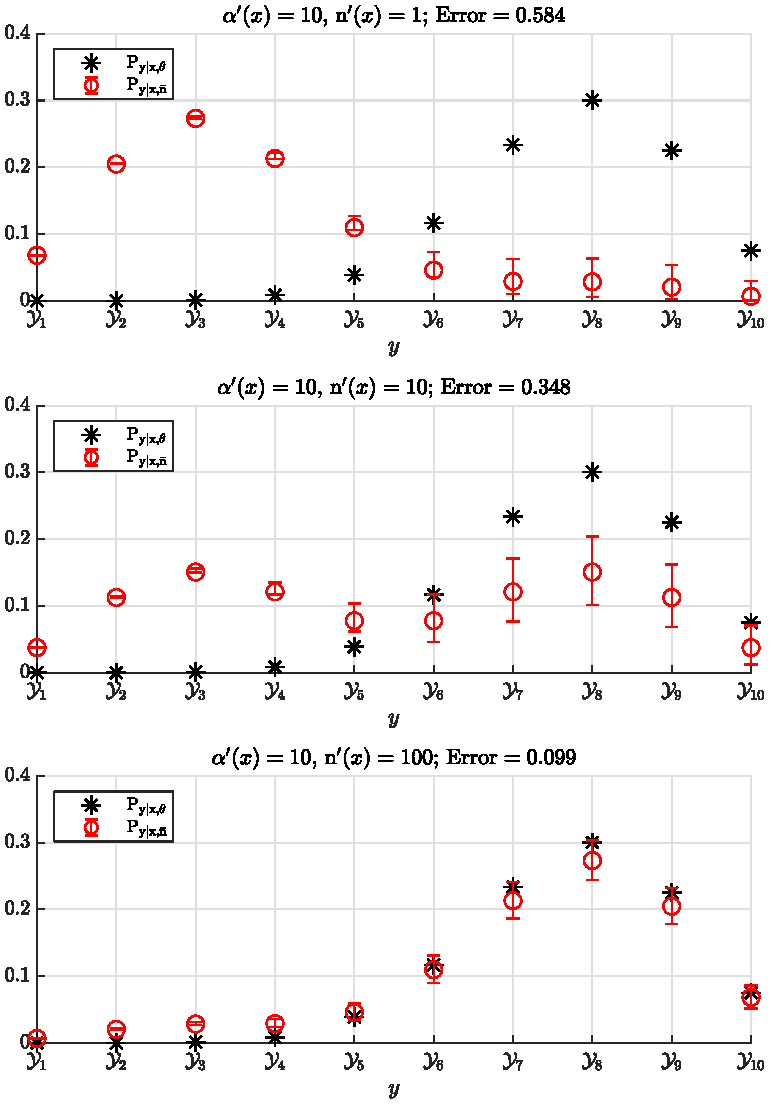
\includegraphics[width=1\linewidth]{P_yx_error_a0_10.pdf}
\caption{Model $\uptheta$ estimates, $\alpha_0 = 10$}
\label{fig:P_yx_error_a0_10}
\end{figure}


The full paper will provide full detail in determining the predictive distributions and expand the discussion on how they are affected by the Dirichlet prior parameters. Additional results will investigate the bias/variance trade-off with other informative examples. The conditional second moments of the difference between the two predicitve PMF's have important applications for Bayesian regression, specifically for determining the expected squared-error loss. This will be a primary focus of future work.






\bibliographystyle{plain}
\bibliography{{../References/phd_bib}}

\end{document}


























